\documentclass{beamer}
\usepackage[utf8]{inputenc}
\usepackage{graphicx}

\title{\textbf{ECSE-487 \\ COMPUTER ARCHITECTURE LABORATORY \\ Assignment \#2}}
\author{Andrei Purcarus Craciun \\ 260631911}
\date{February 13, 2017}

\begin{document}

\maketitle

\begin{frame}
\frametitle{Ripple-carry Frequency Synthesizer}

\begin{itemize}
    \item Data hazards on Cout
    \item Add a register to eliminate hazards at output
\end{itemize}

\begin{figure}[!htb]
    \centering
    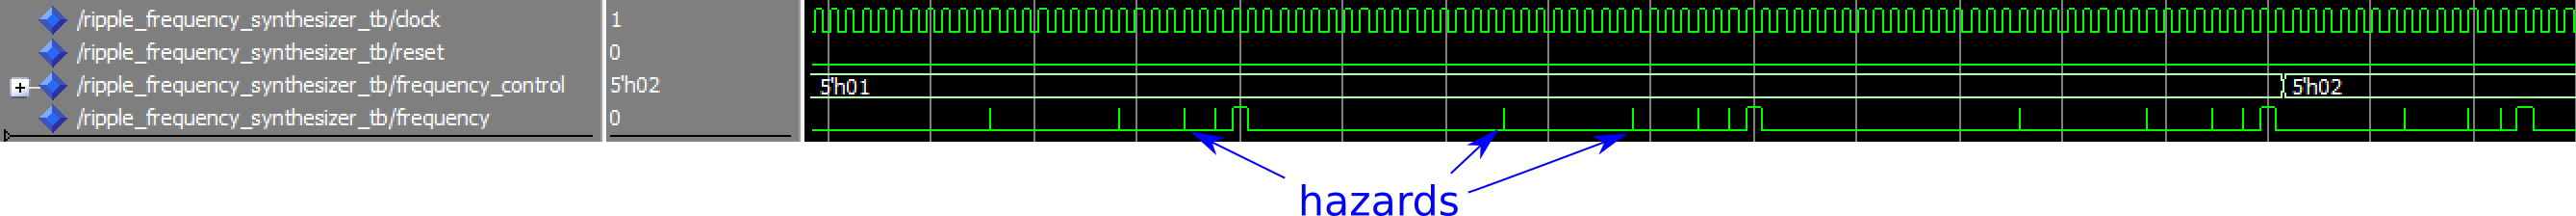
\includegraphics[width=\linewidth]{cout_hazard.PNG}
\end{figure}

\end{frame}

\begin{frame}
\frametitle{Ripple-carry Frequency Synthesizer}

\begin{itemize}
    \item Results
\end{itemize}

\begin{figure}[!htb]
    \centering
    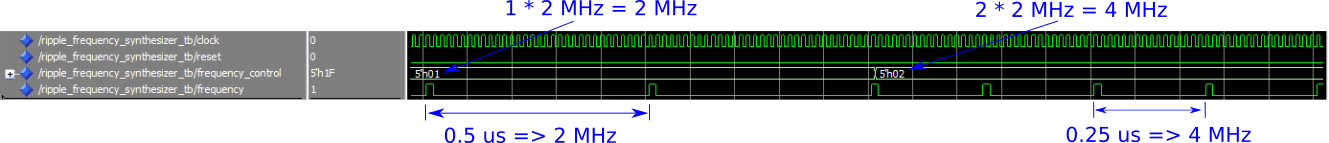
\includegraphics[width=\linewidth]{ripple_2_4_MHz.PNG}
\end{figure}
\begin{figure}[!htb]
    \centering
    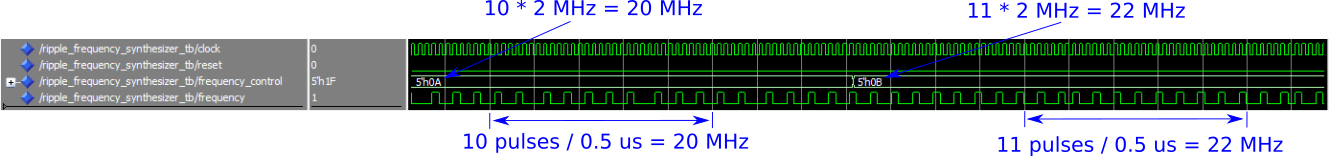
\includegraphics[width=\linewidth]{ripple_20_22_MHz.PNG}
\end{figure}
\begin{figure}[!htb]
    \centering
    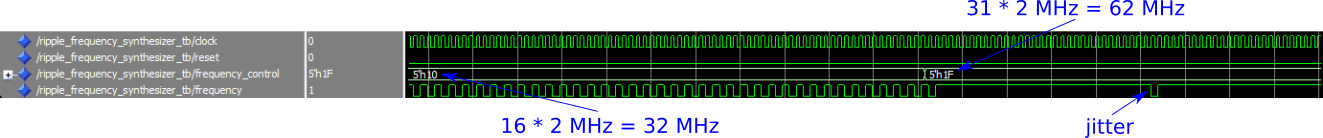
\includegraphics[width=\linewidth]{ripple_32_62_MHz.PNG}
\end{figure}

\end{frame}

\begin{frame}
\frametitle{Ripple-carry Frequency Synthesizer}

\begin{itemize}
    \item Only divisors of clock rate can be generated exactly
    \item Other frequencies experience jitter
\end{itemize}

\[ f_{out} = frequency\_control * \frac{f_{clk}}{N} \]

\begin{figure}[!htb]
    \centering
    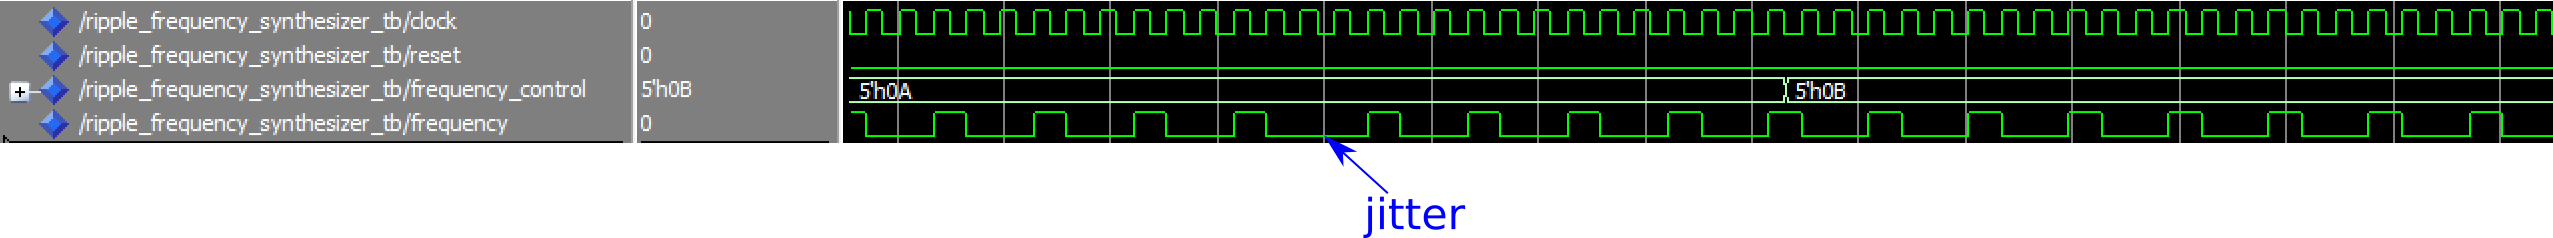
\includegraphics[width=\linewidth]{remainder_jitter.PNG}
\end{figure}

\end{frame}

\begin{frame}
\frametitle{Pipelined Frequency Synthesizer}

\begin{itemize}
    \item Results
\end{itemize}

\begin{figure}[!htb]
    \centering
    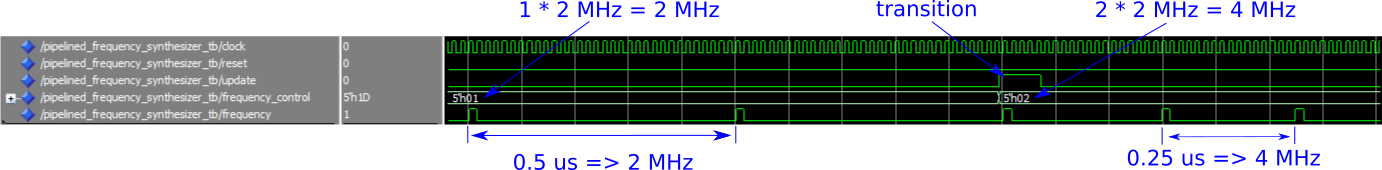
\includegraphics[width=\linewidth]{pipeline_2_4_MHz.PNG}
\end{figure}
\begin{figure}[!htb]
    \centering
    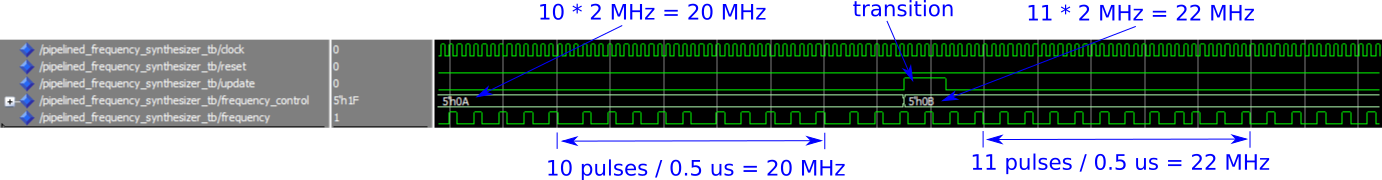
\includegraphics[width=\linewidth]{pipeline_20_22_MHz.PNG}
\end{figure}
\begin{figure}[!htb]
    \centering
    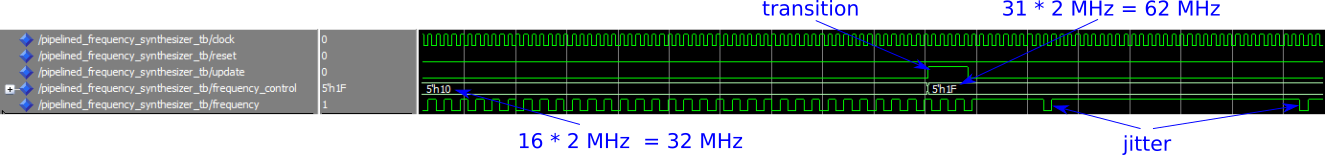
\includegraphics[width=\linewidth]{pipeline_32_62_MHz.PNG}
\end{figure}

\end{frame}

\begin{frame}
\frametitle{Pipelined Frequency Synthesizer}

\begin{itemize}
    \item Synthesis results
    \item Pipelining has more impact with higher N
\end{itemize}

\begin{table}[!htb]
    \centering
    \begin{tabular}[c]{ l | c | c }
        & \textbf{N = 5} & \textbf{N = 32} \\
        \hline
        \textbf{ripple-carry} & 142.71 MHz & 112.23 MHz \\
        \hline
        \textbf{pipelined} & 149.37 MHz & 144.01 MHz \\
    \end{tabular}
\end{table}

\end{frame}

\begin{frame}
\frametitle{FSK Modulator}

\begin{itemize}
    \item Results
\end{itemize}

\begin{figure}[!htb]
    \centering
    \includegraphics[width=\linewidth]{fsk_10_11_MHz.PNG}
\end{figure}
\begin{figure}[!htb]
    \centering
    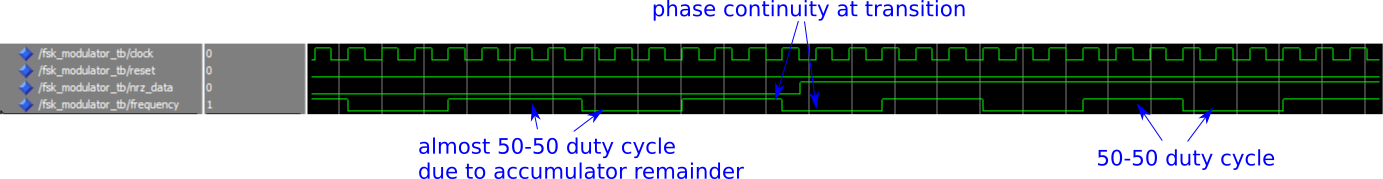
\includegraphics[width=\linewidth]{fsk_50-50_phase.PNG}
\end{figure}

\end{frame}

\begin{frame}
\frametitle{Analog Waveform Generator}

\begin{itemize}
    \item Sine wave shifted to [0, 256)
    \item Results
\end{itemize}

\[ 128 (1 + sin(\frac{2 \pi}{10} t)), t = 0, 1, \ldots 9 \]

\begin{figure}[!htb]
    \centering
    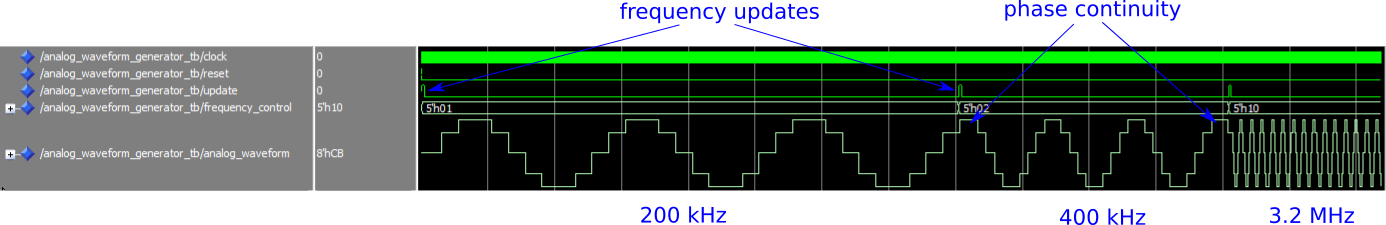
\includegraphics[width=\linewidth]{analog.PNG}
\end{figure}

\end{frame}

\end{document}
